%%%%%%%%%%%%%%%%%%%%%%%%%%%%%%%Section 4%%%%%%%%%%%%%%%%%%%%%%%%%%%%%%%%%%% 

\section{Multiple Linear Regression}\label{sec:MLR}
In sections \ref{sec:Hyp.Testing} and \ref{sec:ANOVA}, we considered a scenario where a single, categorical, explanatory variable (Treatment $A$ vs. Treatment $B$) was used to model a desired response variable (score $y$). Real-world data is, of course, much more intricate and complex, typically consisting of multiple response variables, with multiple quantitative and categorical/qualitative explanatory features. In this section, we will review how such cases can be handled.

\subsection{Multiple Linear Regression in Matrix Form}
Throughout, we suppose that the dataset consists of $N$ observations with a single response output $Y$ and $p$ explanatory variables $X_1,\ldots,X_p$. The \textbf{first-order linear model} describing this scenario can be represented in matrix from by 
\begin{equation}\label{eq:MLR}
    \bm{y}=\bm{X\beta}+\bm{\varepsilon},
\end{equation}
where $\bm{y}=[y_{1},\cdots,y_{N}]^{\!\top}$, $\bm{\beta}=[\beta_{0},\cdots,\beta_{p}]^{\!\top}$, and $\bm{\varepsilon}=[\varepsilon_{1},\cdots,\varepsilon_{N}]^{\!\top}$ are the \textbf{response vector},  the \textbf{coefficient vector}, and  the \textbf{error vector}, respectively, and 
\begin{gather*}
 \bm{X} =  
    \begin{bmatrix}
    1 & x_{1,1} & \cdots & x_{1,p}\\
    1 & x_{2,1} & \cdots & x_{2,p}\\
    \vdots & \vdots & \ddots & \vdots\\
    1 & x_{N,1} & \cdots & x_{N,p}\\
    \end{bmatrix}  
\end{gather*}
is the \textbf{design matrix}, with the further assumption that $\bm{\varepsilon}\sim \mathcal{N}(\bm{0}, \sigma^{2}\bm{I}_n)$, where $\bm{I}$ is the $N \times N$ \textbf{identity matrix}. 

\subsection{Qualitative Explanatory Variables}
It has been said that the colour of a vehicle is part of the assessment for car insurance premiums (whether this is true or not, we are not qualified to discuss). Such a variable is \textbf{qualitative} (nominal, in fact) in nature, as there is no reasonable way to order colours for insurance purposes. If we want to incorporate this feature in an insurance premium model taking into account $k$ possible colour choices, then we need $k-1$ dummy variables $X_1,\ldots,X_{k-1}$ defined according to  the form of
\begin{align*}
    X_{1} &= 
    \begin{cases}
    1 & \text{if colour $=$ red}\\
    0 & \text{otherwise}
    \end{cases}\\
    X_{2} &= 
    \begin{cases}
    1 & \text{if colour $=$ black}\\
    0 & \text{otherwise}
    \end{cases}\\
    & \vdots\\
    X_{k-1} &= 
    \begin{cases}
    1 & \text{if colour $=$ forest green}\\
    0 & \text{otherwise}
    \end{cases}
\end{align*}
With \textbf{ordinal variables} (e.g., \textit{on scale of 1 to 5, how likely are you to buy a new phone this year?}), we may choose to have 4 dummy variables as above, or a single continuous variable. While the latter approach saves 4 degrees of freedom, we are imposing an assumption that equal spacings on the ordinal have an equal impact on the outcome, which is not always the case -- in which case dummy variables might be indicated.

     \begin{table}[!t]
         \centering
         \begin{tabular}{c c c c c}
         \hline
        \textbf{Source} & \textbf{Sum of Squares} & \textbf{d.f.} & \textbf{Mean Square} & $\mathbf{F_{0}}$ \\
         \hline
         Regression & $\text{SS}_{\textrm{reg}}$ & $p-1$ & $\text{MS}_{\textrm{reg}}=\text{SS}_{\textrm{reg}}/(p-1)$ & $\text{MS}_{\textrm{reg}}/\text{MS}_{\textrm{e}}$\\
         Error & $\text{SS}_{\textrm{e}}$ & $N-p$ & $\text{MS}_{\textrm{e}}=\text{SS}_{\textrm{e}}/(N-p)$ \\
         Total & $\text{SS}_{\textrm{tot}}$ & $N-1$\\
        \hline
         \end{tabular}
         \caption[\small ANOVA table for first-order multiple regression]{\small ANOVA table for first-order multiple regression model (\ref{eq:MLR}); with $p$ explanatory variables and $N$ observations. }
         \label{tab:SA4}\hrule
     \end{table}
\subsection{Overall Significance of the Model}
For the model presented in (\ref{eq:MLR}), \textbf{ordinary least square} (OLS) estimation yields \textbf{fitted values} $$\bm{\hat{y}}=\bm{X\hat{\beta}}=\bm{X}(\bm{XX}^{\!\top})^{-1}\bm{X}^{\!\top}\bm{y}$$ and residuals $$\bm{e}=\bm{y}-\bm{\hat{y}}=(\bm{I}-\bm{X}(\bm{XX}^{\!\top})^{-1}\bm{X}^{\!\top})\bm{y}.$$ The ANOVA table has the same form as Table~\ref{tab:SA2} (see Table~\ref{tab:SA4}); it is used in testing $$H_{0}: \beta_{1} = \beta_{2} = \cdots = \beta_{p}=0\quad\mbox{against}\quad H_{1}: \beta_{i} \neq 0 \text{ for at least one  } i.$$ If the test statistic $F_{0}$ is \textbf{significant}, it does not necessarily imply that all the independent variables $X_1, \ldots, X_p$ are useful in predicting $\mathbf{y}$, only that at least one of them is. We can examine significance of the $\beta$ coefficients individually (using $t$-test), or multiple coefficients simultaneously (e.g., \textbf{Bonferroni simultaneous confidence interval}). Choosing the best subset of the model will be discussed in Sections \ref{sec:Data.Red} and \ref{sec:DSML}.

\subsection{Model Adequacy Checks} There are some rare examples for which OLS does not yield a unique solution; but in the vast majority of instances, the data can be fitted to the model. How can we tell if the model is \textbf{adequate} to the situation at hand? 
\begin{itemize}
\item \textbf{Assumptions on Residuals} -- We cannot emphasise enough that \textbf{the model is not necessarily valid when it is statistically significant} (i.e. when $F_0$ is in the critical region); the conclusion only follows once the model has been determined to be an \textbf{adequate} fit for the data. A normal-QQ plot can help verify the assumption of normality, for instance, while the assumptions of independence and constant variance can be tested using scatterplots of fitted values against residuals.

\item \textbf{Outliers and Influential Points} -- In addition, \textbf{outliers} and \textbf{influential points} could affect the fitted values. While it is typically easier to classify some observations as outliers, influential points can distort the regression line significantly. Figure \ref{fig:testA5} shows the clear impact of an influential point. Outliers and influential points should be studied carefully, as there are a number of possible mechanisms that can account for their presence; it may be that these anomalies are due to data entry error, in which case we may try to correct/impute with a reasonable alternative, if possible (see Section~\ref{sec:DP}). It may be the case that these unusual observations are worth studying on their own merit.

\begin{figure}[!t]
\centering
  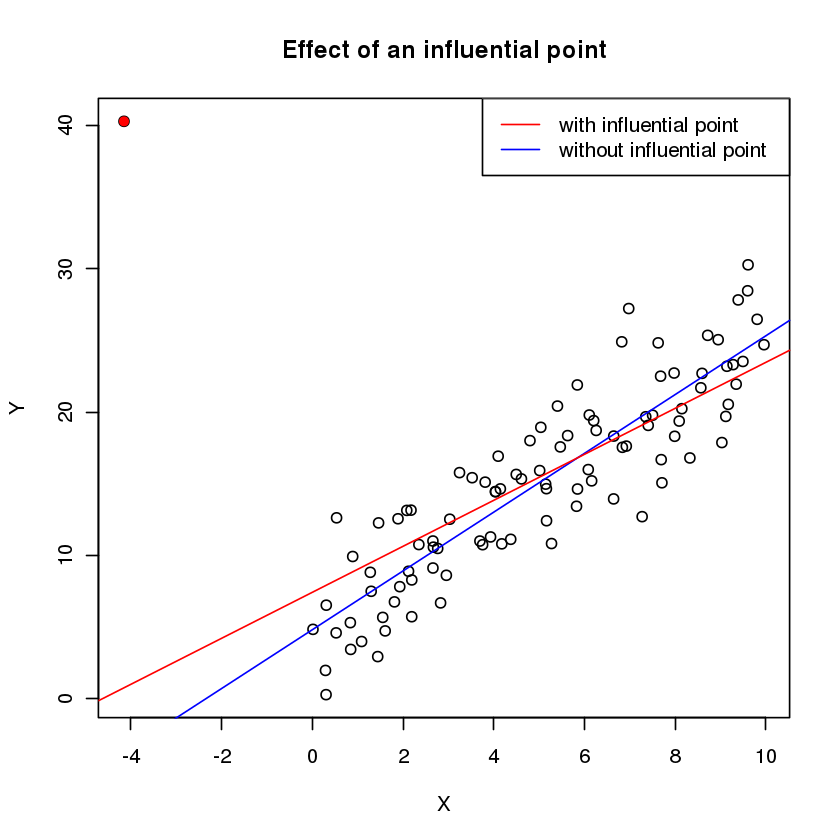
\includegraphics[width=0.5\linewidth]{Images/testA5.png}
  \caption[\small Illustrative example of the effect of an influential point]{\small Illustrative example of the effect of an influential point. The red dot in the top left corner is an influential point -- the slope of the  regression line when it is included in the data (red) is quite different from the slope when it is not (blue).}
  \label{fig:testA5}\hrule
\end{figure}

\item \textbf{Multicollinearity} and \textbf{Variance Inflation Factor} (VIF) -- Last but not least, it is important to take a look at the scatterplot matrix and the correlation matrix of the explanatory variables to detect \textbf{multicollinearity}. While it is hoped that the explanatory variables have some relationship with the response variable (otherwise any model is bound to be fruitless), high correlations and/or dependencies among the explanatory variables is contraindicated as it introduces instability in the estimates of the regression coefficients are unstable. We can formally test for presence of multicollinearity using \textbf{variance inflation factors} (VIF); in its presence, data reduction and data transformation strategies might need to be implemented. 
\end{itemize}


%%%%%%%%%%%%%%%%%%%%%%%%%%%%%%%Section 5%%%%%%%%%%%%%%%%%%%%%%%%%%%%%%%%%%% 

\section{Data Reduction/Model Selection} \label{sec:Data.Red}
In a good model, a balance has been struck between its \textbf{predictive ability} and its \textbf{simplicity}. Clients look for the \textbf{simplest model} that explains the behaviour of the response variable $Y$ in a \textbf{reasonably adequate manner} (a version of \textit{Occam's Razor}). If there are $p$ predictor variables $X_1,\ldots,X_p$, then there are $2^{p}$ possible models from which to select the "best", ranging from the \textbf{simple average model} ${y}_{i}=\beta_{0}+\varepsilon_{i}$ to the \textbf{full model} ${y}_{i}=\beta_{0}+\sum_{j=1}^{p}\beta_{j}x_{i,j}+\varepsilon_{i}$.

\subsection{Step-wise Regression}
As the number of predictors $p$ grows, it is not feasible to fit all $2^{p}$ possible models to determine the optimal model. \textbf{Step-wise regression} is an automated model selection procedure that builds a succession of models from which a choice can be made. There are numerous variants -- this particular algorithm is called \textbf{forward selection}, for reasons that will shortly become clear (to fix the problem in conceptual space, assume that there are $p=10$ predictor variables).
\begin{enumerate}
    \item \textbf{Selecting the first variable:} Fit $p$ simple linear regressions $$y_i=\beta_0 + \beta_jx_{i,j}+\varepsilon_i,\quad j=1,\ldots, p$$ and choose the model with highest $R^{2}$ value. In other words, select the variable $X_j$ that best describes the behaviour of $Y$ \textbf{on its own}. If $X_{5}$ turns out to be that variable, for instance, then the tentative model is $$y_{i}=\beta_{0}+\beta_{5}X_{i,5}+\varepsilon_{i}.$$ If this model is not statistically significant (tested at predetermined significance level $\alpha$), then the final model selection is $$y_{i}=\beta_{0}+\varepsilon_{i}$$ and the search is complete. Otherwise, proceed to step 2.
    \item \textbf{Selecting the second variable:} Fit all two-parameter regression models $$y_i=\beta_0 + \beta_5x_{i,5}+ \beta_jx_{i,j}+\varepsilon_i,\quad j=1,\ldots, p,\quad j\neq 5.$$ Select the model that has the highest value of the test statistic $$t{'}_{k}=\sqrt{\frac{\textrm{MSR}(X_{k}|X_{5})}{\textrm{MSE}(X_{5}, X_{k})}}.$$ Say that $k=3$ yields the largest such value. If the associated model's $p-$value is smaller than $\alpha$, then our tentative model is updated to $$y_{i}=\beta_{0}+\beta_{3}X_{i,3}+\beta_{5}X_{i,5}+\varepsilon_{i}$$ and we proceed to step 3. Otherwise, the final model selection is $$y_{i}=\beta_{0}+\beta_{5}X_{i,5}+\varepsilon_{i}$$ and the search is complete.  
    \item \textbf{All subsequent steps:} Repeat step 2 using $$t^{''}_k=\sqrt{\frac{\textrm{MSR}(X_{k}|X_{5},X_3)}{\textrm{MSE}(X_{5}, X_3,X_{k})}}$$ and so forth, until no additional term improves the model significantly.
\end{enumerate}
In contrast to forward selection which starts with the simple average model $$y_{i}=\beta_{0}+\varepsilon_{i}$$ and build a nested sequence of increasingly complex models, \textbf{backward elimination} begins with the full model $${y}_{i}=\beta_{0}+\sum_{j=1}^{p}\beta_{j}x_{i,j}+\varepsilon_{i}$$ and keeps removing terms until removal of \textit{any} variable causes a significant loss of its predictive power (calculated using $t^{(\ell)}_{k}$). In general, forward selection and backward elimination will not select the same final model. 
\newpage\noindent
In the \textbf{combined approach}, the process starts from the simple average model as in forward selection, but each time a new variable is added to the tentative model, a backward elimination search is performed to test whether any of the previously added variables are no longer significant. This approach enables the model to be better tuned to the data and has been known to prevent \textbf{overfitting} (more on this in Section~\ref{sec:DSML}). In either case, the step-wise selection methods are \textbf{expensive}, computing-wise. 
\newl The test statistic $t^{(\ell)}_{k}$ is the square root of the ratio of conditional MSR over MSE. In everyday terms, it is testing \textit{whether the addition of $X_{k}$ provides a significant improvement in predictive ability over the current tentative model's}. Other alternative include the \textbf{Akaike Information Criterion} (AIC), the \textbf{Bayesian Information Criteria} (BIC), \textbf{Mallow's $\bm{C_{p}}$ Criterion}, and the \textbf{$\bm{R^2}$ criterion} -- simply pick the model which optimises the desired criterion. \newl \textbf{IMPORTANT NOTE:} step-wise regression is \textbf{flawed} in many ways which we will not explore at the moment; in practice, it has slowly started being replaced by \textbf{regularisation methods} such as ridge regression and the LASSO (see Section~\ref{sec:DSML}). From a consulting standpoint, this is a development over which it is worth trying to educate clients. 

%%%%%%%%%%%%%%%%%%%%%%%%%%%%%%%Section 6%%%%%%%%%%%%%%%%%%%%%%%%%%%%%%%%%%% 

\section{Basics of Multivariate Statistics}\label{sec: Multi.Stat}
Up until this point, we have been considering situations the response has been \textbf{univariate}. In applications, especially those that require data science methods, the situation often calls for \textbf{multivariate} responses,  where the response variables are thought to have some relationship (e.g. a \textbf{correlation structure}). It remains possible to analyse each response variable independently, but the dependence structure can be exploited to make \textbf{joint} (or simultaneous) inferences.

\subsection{Properties of the Multivariate Normal Distribution}
The probability density function of a random vector $\mathbf{X}\in\mathbb{R}^p$ that follows a \textbf{multivariate normal distribution} with \textbf{mean vector} $\bm{\mu}$ and \textbf{covariance matrix} $\bm{\Sigma}$, denoted by $\bm{X}\sim\mathcal{N}_p(\bm{\mu},\bm{\Sigma})$, is given by 
\begin{equation*}
f(\bm{X})=\frac{1}{(2\pi)^{p/2}|\bm{\Sigma}|^{1/2}}e^{-\frac{1}{2}(\bm{X}-\bm{\mu})^{\!\top}\bm{\Sigma}^{-1}(\bm{X}-\bm{\mu})},
\end{equation*}
where
\begin{gather*}
    \bm{\Sigma}=
    \begin{bmatrix}
    \sigma_{1,1} & \sigma_{1,2} & \cdots & \sigma_{1,p}\\
    \sigma_{2,1} & \sigma_{2,2} & \cdots & \sigma_{2,p}\\
    \vdots & \vdots &  \ddots & \vdots\\
    \sigma_{p,1} & \sigma_{p,2} & \cdots & \sigma_{p,p}\\
    \end{bmatrix}.  
\end{gather*}
For such an $\bm{X}$, the following properties hold:
\begin{enumerate}[noitemsep]
    \item any linear combination of its components are normally distributed;
    \item all subsets of components follow a (modified) multivariate normal distribution;
    \item a diagonal covariance matrix implies the independence of its components;
    \item conditional distributions of components follow a normal distribution, and 
    \item the quantity $(\bm{X}-\bm{\mu})^{\!\top}\bm{\Sigma}^{-1}(\bm{X}-\bm{\mu})$ follows a $\chi^{2}_{p}$ distribution.
\end{enumerate}
These properties make the multivariate normal distribution attractive, from a theoretical point of view (if not entirely realistic). For instance, 
\begin{itemize}[noitemsep]
\item using the first property, we can use \textbf{contrasts} to test which components are distinct from the others; \item the fifth property is the multivariate analogue of the square of a standard normal random variable $Z\sim\mathcal{N}(0,1)$ following a $Z^2\sim \chi^2_1$ distribution;
\item but two univariate normal random variables with zero covariance are not necessarly independent (the joint p.d.f. of two such variables is not necessarily the p.d.f. of a multivariate normal distribution).
\end{itemize}
A number of univariate approaches generalise nicely. 
\subsection{Hypothesis Testing for Mean Vectors}
When the sample comes from a univariate normal distribution, we can test $$H_{0}: \mu=\mu_{0}\quad\mbox{against}\quad H_{1}: \mu \neq \mu_{0}$$ by using a $t-$statistic. Analogously, if the sample comes from a $p-$variate normal distribution, we can test $$H_{0}: \bm{\mu}=\bm{\mu_{0}}\quad\mbox{against}\quad H_{1}: \bm{\mu} \neq \bm{\mu_{0}}$$ by using \textbf{Hotelling's $\bm{T}^2$ test statistic}, mathematically  defined as
\begin{equation*}
    T^{2}=N\cdot (\bm{\bar{X}}-\bm{\mu})^{\!\top}\bm{S}^{-1}(\bm{\bar{X}}-\bm{\mu})
\end{equation*}
where $\bm{\bar{X}}$ denotes the \textbf{sample mean} and $\bm{S}$ is the \textbf{sample covariance matrix}.
Under $H_{0}$, $$T^{2}\sim \frac{(N-1)p}{(N-p)}F_{p, N-p}.$$ Thus, we do not reject $H_{0}$ at a significance level of $\alpha$ if 
\begin{equation}\label{eq:T2}
    N\cdot (\bm{\bar{X}}-\bm{\mu_{0}})^{\!\top}\bm{S}^{-1}(\bm{\bar{X}}-\bm{\mu_{0}}) \leq \frac{(N-1)p}{(N-p)}F_{p, N-p}(\alpha)
\end{equation}
and reject it otherwise.
\subsection[Confidence Region and Simultaneous Confidence Intervals]{Confidence Region and Simultaneous Confidence Intervals for Mean Vectors}
In the $p-$variate normal distribution, any $\bm{\mu}$ that satisfies the condition
\begin{equation}\label{eq:T2.2}
    N\cdot (\bm{\bar{X}}-\bm{\mu})^{\!\top}\bm{S}^{-1}(\bm{\bar{X}}-\bm{\mu}) \leq \frac{(N-1)p}{(N-p)}F_{p, N-p}(\alpha)
\end{equation}
resides inside a $(1-\alpha)100\%$ \textbf{confidence region} (an ellipsoid in this case). \textbf{Simultaneous Bonferroni confidence intervals} with overall error rate $\alpha$ can also be derived, using 
\begin{equation*}
    (\bar{x}_{j}-\mu_{j})\pm t_{N-1}(\alpha/p)\sqrt{\frac{s_{j,j}}{N}} \text{ for $j=1,\ldots, p$}
\end{equation*}
\newpage\noindent Another approach is to use \textbf{Hotelling's $\bm{T}^2$ simultaneous confidence intervals}, given by 
\begin{equation*}
    (\bar{x}_{j}-\mu_{j})\pm \sqrt{\frac{p(N-1)}{N-p}F_{p,N-p}(\alpha)} \sqrt{\frac{s_{j,j}}{N}} \text{ for $j=1,\ldots, p$}
\end{equation*}
Figure \ref{fig:testA7} shows these regions for a bivariate normal random sample. Notice that the Hotelling's ${T}^{2}$ simultaneous confidence intervals form a rectangle that confines the confidence region, while the Bonferroni confidence intervals are slightly narrower. Given that all the components of the mean vector are correlated (according to a generally non-diagonal covariance matrix), the confidence region should be used if the goal is to study the \textbf{plausibility of the mean vector as a whole}, while Bonferroni confidence intervals may be more suitable when \textbf{component-wise confidence intervals} are of interest. 

\begin{figure}[!t]
\centering
  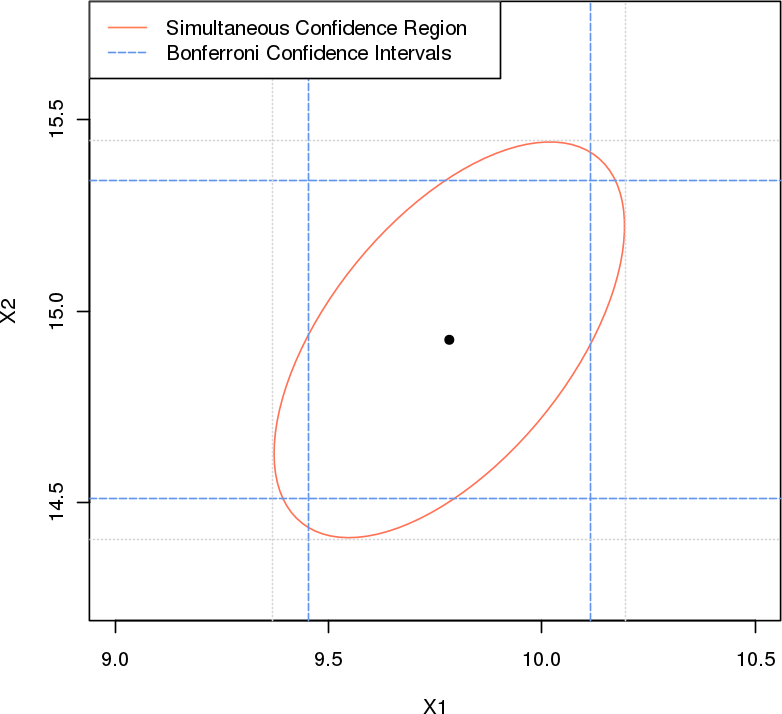
\includegraphics[width=0.5\linewidth]{Images/testA7.png}
  \caption[\small Confidence regions, Bonferroni and Hotelling simultaneous confidence intervals]{\small $95\%$ confidence ellipse, Bonferroni and Hotelling's ${T}^{2}$ simulatenous confidence intervals for a bivariate normal random sample.}
  \label{fig:testA7}\hrule
\end{figure}
\afterpage{\FloatBarrier}

%%%%%%%%%%%%%%%%%%%%%%%%%%%%%%%Section 7%%%%%%%%%%%%%%%%%%%%%%%%%%%%%%%%%%% 

\section{Multivariate Analysis of Variance (MANOVA)}
As shown in Section \ref{sec:ANOVA}, ANOVA is often used in a first pass to determine whether the means from every sub-population are identical.
\subsection{One-Way MANOVA}
ANOVA can test means from more than two populations; the \textbf{multivariate ANOVA} (MANOVA) is quite simply a multivariate extension of ANOVA which tests whether the mean vectors from all sub-populations are identical.
\newl Let there be $I$ sub-populations in the population, from each of which $N_i$ $p-$dimensional responses are drawn, $i=1,\ldots,I$. Mathematically, each observation can be expressed as:
\begin{equation*}
    \bm{X}_{i,j}=\bm{\mu}+\bm{\tau}_{i}+\bm{\varepsilon}_{ij}
\end{equation*}
where $\bm{\mu}$ is the \textbf{overall mean vector}, $\bm{\tau}_{i}$ is the $i^{\text{th}}$ \textbf{population-specific treatment effect}, and $\bm{\varepsilon}_{ij}$ is the \textbf{random error}, which follows a $\mathcal{N}_{p}(\bm{0},\bm{\Sigma})$ distribution. It is important to note that the covariance matrix $\bm{\Sigma}$ is assumed to be the same for each sub-population, and that  $$\sum_{i=1}^{I}N_{i}\bm{\tau}_{i}=\bm{0}$$ to ensure that the estimates are uniquely identifiable.\newl  To test the hypothesis $$H_{0}: \bm{\tau}_{1}=\cdots=\bm{\tau}_{I}=\bm{0}\quad\mbox{against}\quad H_{1}: \text{at least one of } \bm{\tau}_{i}\neq \bm{0},$$ we decompose the total sum of squares and cross-products $\textrm{SSP}_{\textrm{tot}}$ into $$\textrm{SSP}_{\textrm{tot}}=\textrm{SSP}_{\textrm{treat}}+\textrm{SSP}_{\textrm{e}}.$$
     \begin{table}[!t]
         \centering
         \begin{tabular}{c c c c c}
         \hline
        \textbf{Source} & \textbf{SSP} & \textbf{d.f.}\\
         \hline
         Treatment & $\bm{B}=\sum_{i=1}^{I}N_{i}(\bm{\bar{X}}_{i}-\bm{\bar{X}})^{\!\top}(\bm{\bar{X}}_{i}-\bm{\bar{X}})$ & $I-1$\\
         Error & $\bm{W}=\sum_{i=1}^{I}\sum_{j=1}^{n_{i}}(\bm{X}_{ij}-\bm{\bar{X}}_{i})^{\!\top}(\bm{X}_{ij}-\bm{\bar{X}}_{i})$ & $\sum_{i=1}^{I}N_{i}-I$\\
         Total & $\bm{B}+\bm{W}=\sum_{i=1}^{I}\sum_{j=1}^{n_{i}}(\bm{X}_{i,j}-\bm{\bar{X}})^{\!\top}(\bm{X}_{i,j}-\bm{\bar{X}})$ & $\sum_{i=1}^{I}N_{i}-1$\\
        \hline
         \end{tabular}
         \caption[\small One-way MANOVA table]{One-way MANOVA table; with $I$ sub-populations.}
         \label{tab:SA5}
     \end{table}
Based on this decomposition, we compute the test statistic known as \textbf{Wilk's lambda} 
\begin{equation*}
    \Lambda^{*}=\frac{|\bm{W}|}{|\bm{B}+\bm{W}|}
\end{equation*}
and reject $H_{0}$ if $\Lambda^{*}$ is too small. 


%%%%%%%%%%%%%%%%%%%%%%%%%%%%%%%Section 8%%%%%%%%%%%%%%%%%%%%%%%%%%%%%%%%%%% 

\section{Goodness-of-Fit Tests}
% Note: this is a completely arbitrary made up example.
A (fictitious) 2017 survey asked a sample of $N=200$ adults between the age of 25 to 35 about their highest educational achievement. The result is summarised in Table \ref{tab:SA6}. In 1997, it was found that $p_1=13\%$ of adults had not complete high school, $p_2=32\%$ had obtained a high school degree but not a post-secondary degree, $p_3=37\%$ had either an undergraduate college or university diploma but no post-graduate degree, and $p_4=18\%$ had at least one post-graduate degree. Based on the result of this survey, is there sufficient evidence to believe that educational backgrounds of the population have changed since 1997?
     \begin{table}[!t]
         \centering
         \begin{tabular}{c c c c}
         \hline
        \textbf{1. Some HS or Less} & \textbf{2. HS} & \textbf{3. College/University} & \textbf{4. Post-Graduate or higher} \\
         \hline
        $16$ & $55$ & $83$ & $46$ \\
        \hline
         \end{tabular}
         \caption[\small Respondents' educational achievements]{\small Respondents' educational achievements, from a (fictitious) 2017 survey.}
         \label{tab:SA6}\hrule 
     \end{table}
\par Since each respondent's educational achievement can only be classified into one of these categories, they are  \textbf{mutually exclusive}. Furthermore, since these categories cover all possibilities on the educational front, they are also \textbf{exhaustive}. We can thus view the distribution of educational achievements as being \textbf{multinomial}. For such a distribution, with parameters $p_{1},\cdots,p_{k}$, the expected frequency in each category is $m_{j}=Np_{j}$. \newl  Let $O_{j}$ denote the observed frequency for the $j^{\text{th}}$ category. If there has been no real change since 1997, we would expect the sum of squared differences between the observed 2017 frequencies and the expected frequencies based on 1997 data to be small. We can use this information to test the \textbf{goodness-of-fit} between the observations and the expected frequencies \textit{via} Pearson's $\chi^{2}$ test statistic 
\begin{equation*}
    X^{2}=\sum_{j=1}^{k}\frac{(O_{j}-m_{j})^{2}}{m_{j}}    
\end{equation*}
which follows a $\chi^{2}$ distribution with $k-1$ degrees of freedom.
\newl In the above example, the hypotheses of interest are $$H_{0}: p_{1}=0.13,p_{2}=0.32,p_{3}=0.37,p_{4}=0.18\quad\mbox{against}\quad H_{1}: \text{not } H_{0}.$$ Table  \ref{tab:SA7} summarises the information under $H_{0}$.
     \begin{table}[!t]
         \centering
         \begin{tabular}{c c c c c}
         \hline
        \textbf{Category} & $\bm{O}_{j}$ & $\bm{p}_{j,0}$ & $\bm{m}_{j,0}$ & $(\bm{O}_{j}-\bm{m}_{j,0})^2/\bm{m}_{j,0}$  \\
         \hline
        $1$ & $16$ & $0.13$ & $26$ & $3.846$ \\
        $2$ & $55$ & $0.32$ & $64$ & $1.266$ \\
        $3$ & $83$ & $0.37$ & $74$ & $1.095$ \\
        $4$ & $46$ & $0.18$ & $36$ & $2.778$ \\
        \hline
        Total & $200$ & $1$ & $200$ & $7.815$\\
        \hline
         \end{tabular}
         \caption[\small Summary table for goodness-of-fit data for educational achievements]{\small Summary table for goodness-of-fit data for educational achievements under $H_0$.}
         \label{tab:SA7}\hrule
     \end{table}
Pearson's test statistic is $X^{2}=7.815$, with an associated $p-$value of $0.0295$, which implies that there is enough statistical  evidence (at the $\alpha=0.05$ level) to accept that the population's educational achievements have changed over the last 20 years.


%%%%%%%%%%%%%%%%%%%%%%%%%%%%%%%Section 9%%%%%%%%%%%%%%%%%%%%%%%%%%%%%%%%%%% 

\section{Analysis of Covariance (ANCOVA)}
In Section \ref{sec:Hyp.Testing}, we looked at the effectiveness of new teaching method by assigning each group to a specific treatment and comparing the mean test scores. A crucial assumption for that model is that subjects in each group have \textbf{similar background knowledge} about statistics prior to the three week lectures. If this assumption is wrong, however, we may be making incorrect decisions based on the model. Even if each group had similar background knowledge \textit{on average}, there may be large variability from person-to-person, masking the true treatment effect.

\subsection{Paired Comparison}
One way to avoid such \textbf{subject-to-subject variability} is to administer both treatments to each individual,  and then compare treatment effects by looking at the \textbf{difference in the outcomes}. If a grocery chain is interested in measuring the effectiveness of two advertising campaigns, for instance, it is reasonable to assume that there is a large variability in total sales, as well as popular items sold, at each store -- it may then be preferable to run both campaigns in each store and analyse the resulting data rather than to split the stores into two groups (in each of which a different advertising campaign is run) and then to compare the mean outcomes in the two groups. 

Formally, let $X_{i,1}$ denote the total sales with campaign $A$ and $X_{i,2}$ the total sales with campaign $B$. The quantity of interest is $D_{i}=X_{i,1}-X_{i,2}$ for each store $i=1,\ldots,N$. Assuming that the differences $D_{i}$ follow an {i.i.d.} normal distribution with mean $\delta$ and variance $\sigma^{2}_{d}$, then we can test $$H_{0}: \delta=0\quad\mbox{against}\quad H_{1}: \delta \neq 0$$ by using the test statistic $$t_0=\sqrt{N}\frac{\bar{D}}{s_{d}},$$ which follows a Student's $t$ distribution with  $N-1$ degrees of freedom; thus we reject $H_{0}$ if the observed test statistic $t_{0}$ has $p$-value less than the pre-specified significance level $\alpha/2$.

\subsection{Analysis of Covariance (ANCOVA)}
ANOVA compares multiple group means and tests whether any of the group means differ from the rest, by breaking down the total variability into a treatment (explainable) variability component and an error (unexplained) variability component, and building a ratio $F_0$ to determine whether or not to reject $H_{0}$. \par \textbf{Analysis of covariance} (ANCOVA) introduces \textbf{concomitant variables} (or \textbf{covariates}) to the ANOVA model, splitting the total variability into 3 components: $\text{SS}_{\textrm{treat}}$, $\text{SS}_{\textrm{con}}$, and $\text{SS}_{\textrm{e}}$, aiming to reduce error variability. The choice of covariates is thus crucial in running a successful ANCOVA.
\newl In order to be useful, a concomitant variable must be related to response variable in some way, otherwise it not only fails to reduce error variability, but it also increases the model complexity. In the teaching method example, we could consider administering a pre-study test to measure the prior knowledge level of each participant and use this score as a concomitant variable. In the advertising campaign example, we could have used the previous month's sales as a covariate. In medical studies, we could use the age and weight of subjects as covariates.
\par But concomitant variables should not be affected by treatments. Suppose that, in a medical study, patients were asked \textit{how strongly they believed that they were given actual medication rather than a placebo}. If the treatment is indeed effective, then a participant's response to this question could be \textbf{markedly different} in the treatment group than in the  placebo group (perhaps the medication has strong side-effects which cannot be ignored). This means that true treatment effect may be masked by concomitant variable due to unequal effects on treatment groups.
\newl Qualitative covariates (such as gender, say) are not part of the ANCOVA framework. Indeed, such a covariate just creates new ANOVA treatment groups. \newl Figure \ref{fig:testA14} shows a potential breakdown of the total variability when moving from an ANOVA to an ANCOVA model -- the error variability is further split into an error and a covariate component, while the treatment variability remains unchanged.
\begin{figure}[!t]
\centering
  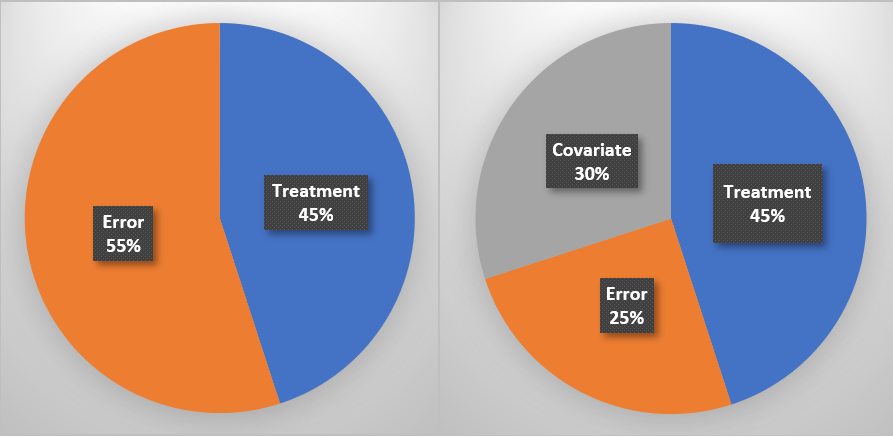
\includegraphics[width=0.6\linewidth]{Images/testA14.png}
  \caption[\small Breakdown of variability for ANOVA and ANCOVA]{\small Breakdown of variability for ANOVA and ANCOVA.}
  \label{fig:testA14}\hrule
\end{figure}
\afterpage{\FloatBarrier}
\subsection{ANCOVA Model and Its Assumptions}
Suppose that we are testing the effect of $p$ treatments, with $N_{j}$ subjects in each group. Then the ANCOVA model takes the form
\begin{equation}\label{eq:ANCOVA}
    y_{i,j}=\mu+\tau_{j}+\gamma (x_{i,j}-\bar{x})+\varepsilon_{i,j}
\end{equation}
where 
\begin{itemize}[noitemsep]
    \item $y_{i,j}$ is the response of the $i^{\text{th}}$ subject in the $j^{\text{th}}$ treatment group;
    \item $\mu$ is the overall mean;
    \item $\tau_{j}$ is the $j^{\text{th}}$ treatment effect subject to a constraint $\sum_{j=1}^{p}\tau_{j}=0$;
    \item $\gamma$ is the coefficient for the \textbf{covariate effect};
    \item $(x_{i,j}-\bar{x})$ is the covariate value of the $i^{\text{th}}$ subject in the $j^{\text{th}}$ treatment group, adjusted by the mean, and
    \item $\varepsilon_{i,j}$ is the error of $i^{\text{th}}$ subject in the $j^{\text{th}}$ treatment group.
\end{itemize}
Four assumptions must be satisfied:
\begin{itemize}[noitemsep]
    \item \textbf{independence and normality of residuals} -- the residuals are thought to follow an ${i.i.d.}$ normal distribution with mean of $0$ and variance $\sigma^{2}_{\varepsilon}$;
    \item \textbf{homogeneity of residual variances} -- the variance of the residuals must be uniform across treatment groups;
    \item \textbf{homogeneity of regression slopes} -- the regression effect (slope) must be uniform across treatment groups, and
    \item \textbf{linearity of regression} -- the regression relationship between the response and the covariate must be linear.
\end{itemize}
The first of these assumptions can be tested with the help of a QQ-plot and a scatter-plot of residuals vs. fitted values, while the second may use the Bartlett or the Levene test. The final assumption is not as crucial as the other three assumptions. Various remedial methods can be applied should any of these assumptions fail.  
\par The third assumption, however, is \textbf{crucial} to the ANCOVA model; it can be tested with the \textbf{equal slope test}, which requires an ANCOVA regression on equation (\ref{eq:ANCOVA}) with an additional interaction term $x \times \tau$. If the interaction is not significant, the third assumption is satisfied. In the event that the interaction term is statistically significant, a different approach (e.g. moderated regression analysis, mediation analysis) is required since using the original ANCOVA model is not prescribed. An in-depth application of an ANCOVA model is highlighted in Section \ref{sec:CCNM}.

%%%%%%%%%%%%%%%%%%%%%%%%%%%%%%%Section 10%%%%%%%%%%%%%%%%%%%%%%%%%%%%%%%%%%% 

\section{Nonlinear Regression}
From the use of tooth paste, cosmetics, cleaning solutions and so forth, we are exposed to numerous chemicals on a daily basis; thousands of new chemicals are introduced into commercial products each year, and government agencies (such as Health Canada and the Environmental Protection Agency in the U.S.) must determine whether these chemicals are safe for humans, animals, and the environment. \par To test whether a chemical poses a risk of adverse effects, we must first determine whether it triggers adverse effects over a range of potential exposure levels, and if so, how much is considered safe (or how much would pose an unacceptable risk). Traditionally (and not necessarily ethically), rodents were used to study whether a chemical is carcinogenic or not.\newl  Suppose that $N$ laboratory rodents are divided into $k$ groups, with each group consisting of $N_{i}$ rodents. Over the course of the experiment, each group was given a certain amount of exposure to the chemical under investigation. The outcome of the experiment is whether each rodent eventually develops a tumour or not; that is, the outcome is expressed as $0$ (tumour absent) or $1$ (tumour present). Table \ref{tab:SA8} summarises the outcome of an experiment. \par Clearly, we cannot fit an ordinary linear regression to the data as the outcome is \textbf{dichotomous}. How could we model the relationship between the adverse effect and the dose levels?

     \begin{table}[!t]
         \centering
         \begin{tabular}{c c c c c}
         \hline
        Dose levels ($d$) & 0 & 7000 & 15000 & 30000\\
        Sample size ($n$) & 50 & 35 & 65 & 50\\
        Number of observed adverse effect ($y$) & 3 & 6 & 33 &39\\
        Rate of observed adverse effect ($p$) & 0.06 & 0.17 & 0.51 & 0.78\\
        \hline
         \end{tabular}
         \caption[\small Summary of experimental results involving C.I. Acid Red 114]{Summary of experimental results involving C.I. Acid Red 114; $N=200$.}
         \label{tab:SA8}
     \end{table}
For each dose level $d$, the probability of adverse effect is $p_{d}=P(y=1|d)$. The \textbf{conditional expectation} given the dose level is also $E(y=1|d)=p_{d}$. Since the relationship resembles an $S-$shaped curve, we may use a  logistic distribution to model the data:
\begin{equation*}
    E(y=1|d)=p_{d}=\frac{\exp[\beta_{0}+\beta_{1}d]}{1+\exp[\beta_{0}+\beta_{1}d]}
\end{equation*}
To obtain \textbf{maximum likelihood estimates} for $\beta_{0}$ and $\beta_{1}$, we need to rely on numerical methods such as the \textbf{Newton-Raphson method}; the dose-response model for the above example is shown in Figure \ref{fig:testA8}.

\begin{figure}[!t]
\centering
  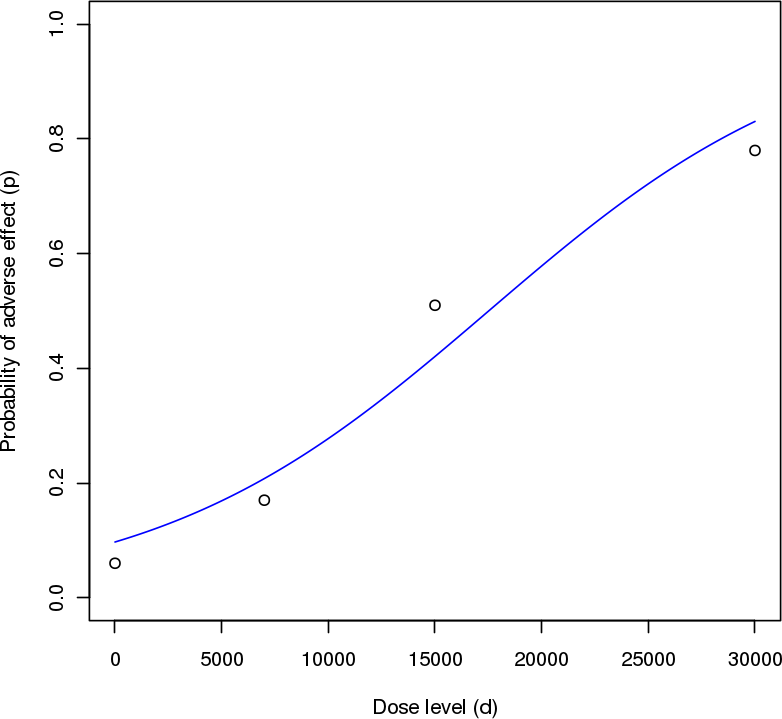
\includegraphics[width=0.5\linewidth]{Images/testA8.png}
  \caption[\small Dose-response model for C.I. Acid Red 114 using logistic regression]{\small Dose-response model for C.I. Acid Red 114 using logistic regression.}
  \label{fig:testA8}\hrule
\end{figure}
\subsection{Relationship to Linear Regression}
Since $p_{d}$ is a probability, it has to lie in $[0,1]$. By taking the odds of having an adverse effect, defined by $\omega_{d}=p_{d}/(1-p_{d})$, the boundary of the response is changed to $[0,\infty)$. Taking the log odds will span $\mathbb{R}$, and the functional form of the \textbf{logistic regression model} is 
\begin{equation} \label{eq:logit}
    \log(\omega_{d})=\log\left(\frac{p_{d}}{1-p_{d}}\right)=\beta_{0}+\beta_{1}d,
\end{equation}
which is a simple linear regression model.

\subsection{Other Non-Linear Regression Models}
Other \textbf{sigmoidal curves} can be used to model the relationship between predictors and a binary response variable. Popular alternatives include the \textbf{probit} link $P(y|x)=\Phi(\beta_{0}+\beta_{1}x)$, where $\Phi$ is the cumulative distribution function of the standard normal distribution, or the \textbf{complementary log-log} link $P(y|x)=1-\exp(-\exp(\beta_{0}+\beta_{1}x))$. In toxicology studies, one of the most widely used model is called the \textbf{Hill}, and it is defined \textit{via} 
\begin{equation*}
    P(y|d,\alpha, \kappa, \eta)=\alpha + (1-\alpha)\frac{d^{\eta}}{d^{\eta}+\kappa^{\eta}};
\end{equation*}
part of its appeal to health scientists is the interpretation of its parameters -- $\alpha$ represents the \textbf{background rate for adverse effect}, while $\kappa$ denotes $\textrm{ED}_{50}$ (the \textbf{effective dose at which $50\%$ of participants would exhibit the response of interest}) and $\eta$ provides the \textbf{steepness of the dose-response curve}. \par Figure \ref{fig:testA9} compares the simple logistic model to the Hill model; we observe that the Hill model provides a closer fit to the observed proportions, and the curvature is more pronounced compared to the logistic model.

\begin{figure}[!t]
\centering
  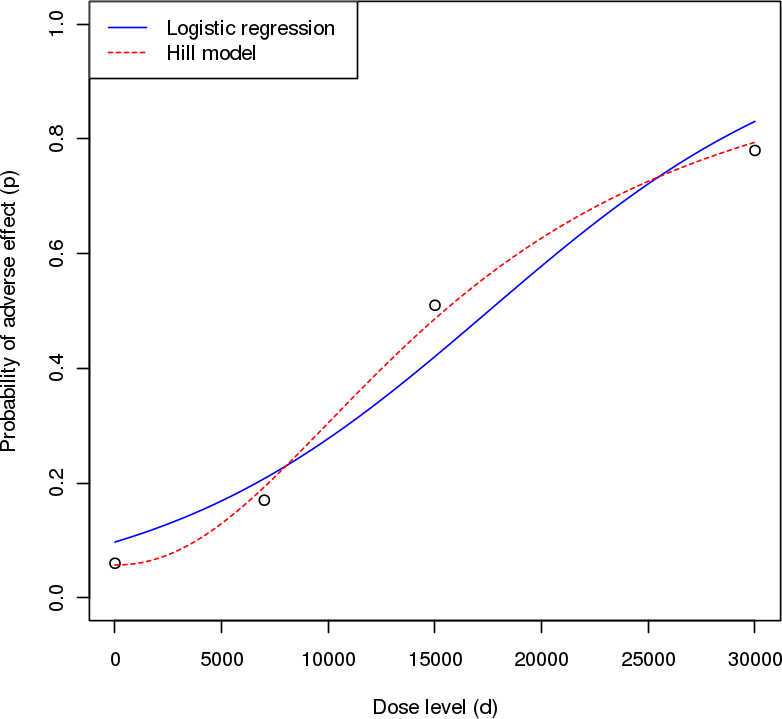
\includegraphics[width=0.5\linewidth]{Images/testA9.png}
  \caption[\small Dose-response model for C.I. Acid Red 114 using the Hill model]{\small Dose-response model for C.I. Acid Red 114 using logistic regression (blue) and the Hill model (red).}
  \label{fig:testA9}\hrule
\end{figure}


%%%%%%%%%%%%%%%%%%%%%%%%%%%%%%%Section 11%%%%%%%%%%%%%%%%%%%%%%%%%%%%%%%%%%% 

\section{Bayesian Statistics}
In classical statistics, model parameters such as $\mu$ and $\sigma$ are treated as constants; \textbf{Bayesian statistics}, on the other hand assume that \textbf{model parameters are random variables}. As the name implies, Bayes' Theorem lies at the foundation of Bayesian statistics: 
\begin{equation}\label{eq:Bayes}
    P(H|D)=\frac{P(D|H)\times P(H)}{P(D)},
\end{equation}
where $H$ represents the hypothesis and $D$ denotes the observed data, which is sometimes written in shorthand as  $\textrm{\textbf{posterior}} = P(H|D) \propto P(D|H)\times P(H) = \textrm{\textbf{evidence}} \times \textrm{\textbf{prior}}.$ In other words, our degree of belief in a hypothesis should be updated by the evidence provided by data. \newpage\noindent \textbf{IMPORTANT NOTE:} the use of Bayesian statistics is controversial in many quarters, and your clients (or fellow consultants) might have strong \textbf{frequentist} leanings. Navigate with care. \begin{center}
    \rule{0.5\textwidth}{.4pt}
\end{center}
Bayes' Theorem escapes the controversy -- nobody disputes its validity -- and has proven to be a useful component in various models and algorithms, such as email spam filters, and the following example. \newl 
Suppose we are interested in diagnosing whether a tumour is begin or malignant, based on several measurements obtained from video imaging. Bayes' Theorem (\ref{eq:Bayes}) can be recast in a tumour data mould:
\begin{itemize}[noitemsep]
    \item \textbf{posterior:} $P(H|D)=$ based on collected data, how likely is a given tumour to be benign (or malignant)?
    \item \textbf{prior:} $P(H)=$ in what proportion are tumours benign (or malignant) in general? 
    \item \textbf{likelihood:} $P(D|H)=$ knowing a tumour is benign (or malignant), how likely is it that these particular measurements would have been observed?
    \item \textbf{evidence:} $P(D)=$ regardless of a tumour being benign or malignant, what is the chance that a tumour has the observed characteristics?
\end{itemize}
To answer the above question (that is, to compute the posterior), we will use a \textbf{na\"{\i}ve Bayes classifier} (see Section~\ref{sec:DSML} for other classification methods).
\subsection{Na\"{\i}ve Bayes Classification for Tumour Diagnoses}
\begin{enumerate}[noitemsep]
    \item \textbf{Objective function:} a simple way to determine whether a tumour is benign or malignant is to compare \textbf{posterior probabilities} and choose the one with highest probability. That is, we diagnose a tumour as \textbf{malignant} if 
        \begin{equation*}
        \frac{P(\textrm{malignant}|D)}{P(\textrm{benign}|D)}=\frac{P(D|\textrm{malignant})\times P(\textrm{malignant})}{P(D|\textrm{benign})\times P(\textrm{benign})}>1,
    \end{equation*}
    and as \textbf{benign} otherwise. 
    
    \item \textbf{Dataset:} the classifier is built on a sample of $N=458$ tumours with nine measurements, each scored on a scale of 1 to 10. The measurements include items such as \textit{clump thickness} and \textit{bare nuclei}; boxplots of these measurements are shown in Figure~\ref{fig:testA10}. We also have one undiagnosed case with these measurements, with its explanatory signature scores given in Table~\ref{fig:testA12}; this is the observation for which a prediction is required.    
    \begin{figure}[!t]
    \centering
      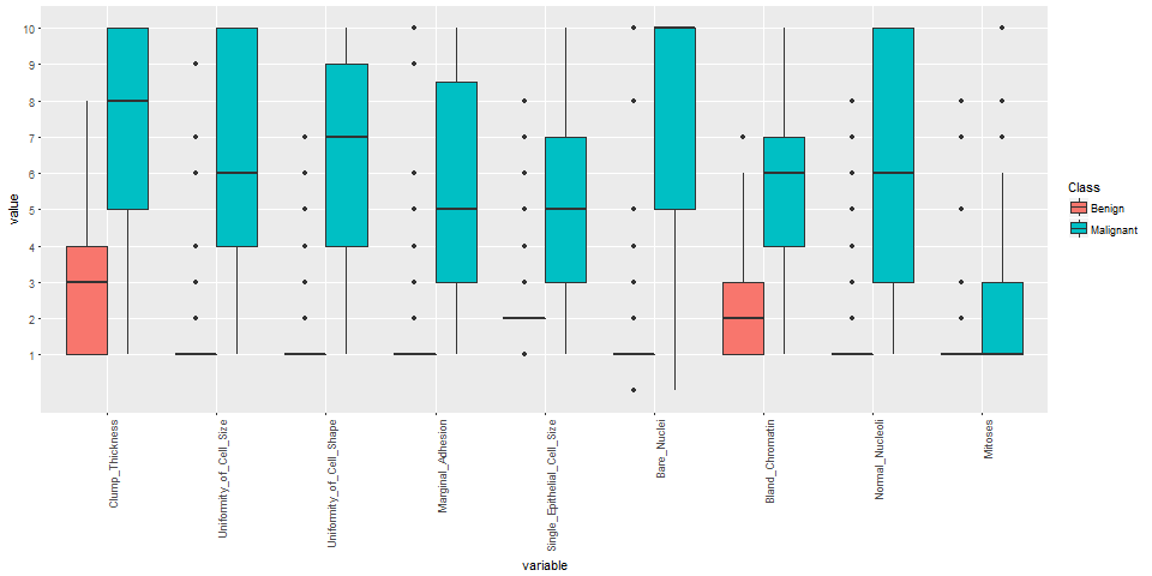
\includegraphics[width=\textwidth]{Images/testA10.png}
      \caption[\small Visualisation of tumour measurements]{\small Boxplot visualisation of measurements for benign and malignant tumours.}
      \label{fig:testA10}
    \end{figure}
    
    \begin{table}[!t]
    \centering
      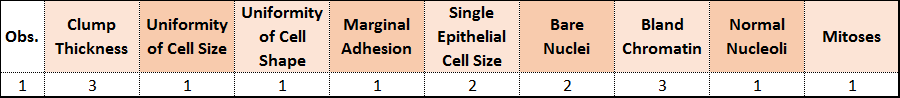
\includegraphics[width=\textwidth]{Images/testA12.png}
      \caption[\small Scores for an undiagnosed tumour]{Scores for an undiagnosed tumour.}
      \label{fig:testA12}\hrule
    \end{table}

    \item \textbf{Assumptions:} we assume that the scores of each measurement are independent of one another (hence the \textit{naive} qualifier); this assumption simplifies the likelihood function to
    \begin{align*}
        P(H|D)=P(H|x_{1},x_{2},\cdots,x_{9})=P(H|x_{1})\times \cdots\times P(H|x_{9}).
    \end{align*}
    \item \textbf{Prior distribution:} we can ask subject matter experts to provide a rough estimate for the general ratio of benign to malignant tumours, or use the proportion of benign tumours in the sample as our prior. In situations where we have no knowledge about this distribution, we may simply assume a \textbf{non-informative prior} (in this case, the prevalence rates being the same for both responses). 
    
    \item \textbf{Computation of likelihoods:} under independence, each measurement is assumed to follow a multinomial distribution (since scores are on scale from 1 to 10). Multiplying probabilities from each multinomial distribution (one each for both classes) provides the overall likelihoods for benign and malignant tumours, respectively. The likelihood of the undiagnosed case being a benign tumour is given to be $9.06\times 10^{-4}$, while the likelihood of being a malignant tumour is $5.85\times 10^{-11}$, based on the multinomial probabilities given in Table~\ref{fig:testA13}
    
    \begin{figure}[!t]
    \centering
      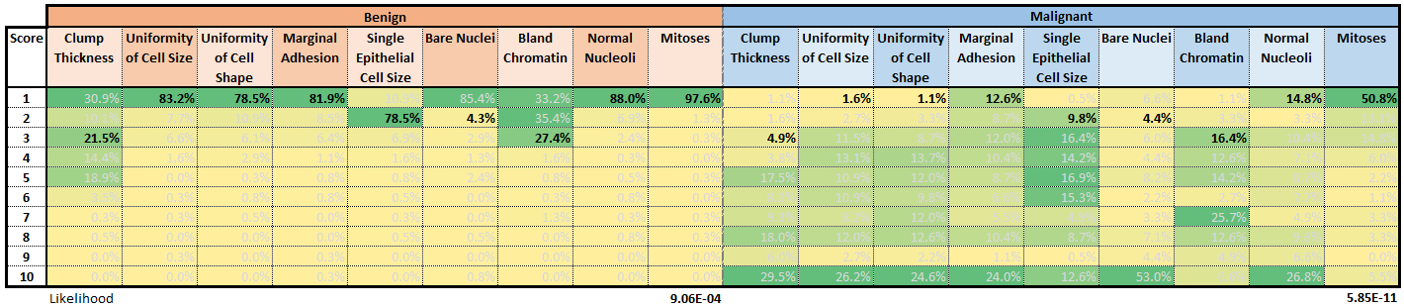
\includegraphics[width=1\linewidth]{Images/testA13.png}
      \caption[\small Multinomial probabilities for benign and malignant tumours]{\small Multinomial probabilities for benign and malignant tumours.}
      \label{fig:testA13}
    \end{figure}
    
    
    \item \textbf{Computation of Posterior:} Multiplying the prior probability and likelihood, we get a quqntity that is proportional to the respective posterior probabilities. Looking at Table \ref{tab:SA9}, we conclude that the tumour in the undiagnosed case is\textbf{likely benign} (note that we have no measurement on how much more likely it is to be benign than to be malignant -- the classifier is \textbf{not calibrated}).
    
    \begin{table}[!t]
        \centering
        \begin{tabular}{c c c c c}
        \hline
        \textbf{Class} & \textbf{Prior} & \textbf{Likelihood} & \textbf{Posterior} & \textbf{Ratio}\\
        \hline
            \textbf{Malignant} & $0.327$ & $5.85\times 10^{-11}$ & $1.92\times 10^{-11}$ & $3.15 \times 10^{-8}$\\
        \textbf{Benign} & $0.673$ & $9.06\times 10^{-4}$ & $6.09\times 10^{-4}$ \\

        \hline
        \end{tabular}
        \caption[\small Computation of posterior probabilities in the undiagnosed case]{Computation of posterior probabilities in the undiagnosed case.}
        \label{tab:SA9}\hrule
     \end{table}    
        
\end{enumerate}

\section[Case Study: ANCOVA for a Clinical Study]{Case Study: Covariance Analysis of the Effect of a Probiotic Agent on IBS}\label{sec:CCNM}
\textbf{Irritable Bowel Syndrome} (IBS) is a functional colonic disease with high prevalence. Typical symptoms include ``chronic abdominal pain, discomfort, bloating, and alteration of bowel habits'' [Wikipedia]; it has been linked to chronic pain, fatigue, and work absenteeism and is considered to have a severe impact on quality of life [Par\'e \textit{et al.} (2006), Maxion-Bergemann \textit{et al.} (2006)]. Although there is no known cure for IBS, there are treatments that attempt to relieve symptoms, including dietary adjustments, medication and psychological interventions.
\par In 2010, the \textit{Canadian College of Naturopathic Medicine} (CCNM) was commissioned to conduct a study to investigate the effect of a probiotic agent on IBS. The study's details and a preliminary data analysis using \textbf{hierarchical linear models} (HLM) can be found in a preliminary report -- it's key findings are that a strong placebo/expectation effect is present in the early stages of the study (which is not entirely surprising given the nature of the phenomenon under study), and that there is no strong statistical evidence to suspect that the agent itself has much of an effect on mild to moderate IBS [Herman, Cooley, Seely (2011)].
\par The sponsor has expressed interest in determining whether these findings still hold when the trial data is examined using \textbf{analysis of covariance} (ANCOVA), a general linear model which evaluates whether the population means of a dependent/response variables (in this case, \textit{IBS Severity} or a measure of \textit{Quality of Life} (QoL)) are equal across levels of a categorical independent variable (in this case, two treatment effects over time), while statistically controlling for the effects of covariates (in this case, the baseline scores for IBSS and QoL). By comparison with the more traditional analysis of variance (ANOVA), ANCOVA can be used to increase the likelihood of finding a significant difference between treatment groups (when one exists) by reducing the within-group error variance.\newl While some of the results looked promising (in particular for severe IBS sufferers), no statistical evidence for treatment effect was found at the 95\% significance level; furthermore, even had evidence been found at that level, design and recruitment issues would have called their practical significance into question. \par In 2013, CCNM conducted a second study to investigate the effect of the probiotic agent, this time focusing on severe IBS. The results are provided in the report ``Covariance Analysis of IBS Study II''. 